\color{white}
\pagecolor{black_background}

\tableofcontents
\newpage

\chapter{SISTEMAS DE LOSAS POSTENSADAS}
\newpage

\section{USO DE LOSAS POSTENSADAS EN EDIFICACIONES}

Esta es una imagen que se hizo en Bolivia, en el departamento de
Potosi. donde se tenia la idea de eliminar las dos columnas marcadas
de color rojo.

\begin{figure}[H]
\centering
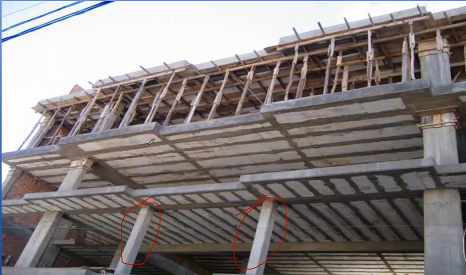
\includegraphics{1.png}
\end{figure}

En la siguiente imagen se muestra un esquema de la primera losa 
de hormigon armado y luego una losa postensada, para precindir 
de las columnas en las losas superiores. Es decir por razones
de funcionalidad se queria hacer salon de fiestas, Es decir que
se tiene que verificar que cumpla con la vibración permitida.

\begin{figure}[H]
\centering
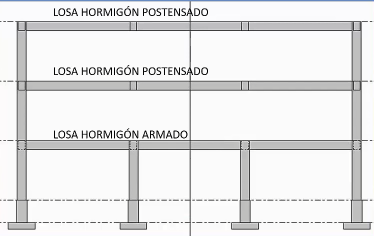
\includegraphics{2.png}
\end{figure}

A travez de los cables y los anclajes se logra generar una carga
opuesta al peso propio. como se muestra en la siguiente imagen

\begin{figure}[H]
\centering
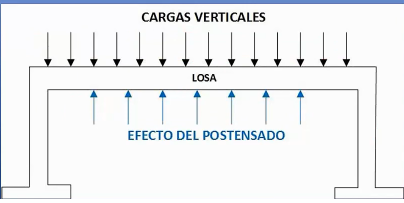
\includegraphics{3.png}
\end{figure}

\section{MATERIALES}

\begin{itemize}
	\item HORMIGON, ACERO (barras corrugadas)
	\item CABLE PARA POSTENSADO
	\item ANCLAJES
\end{itemize}

En la siguiente imagen se muestra el cable para puentes, que coloquialmente
le decimos cable pelado. La tecnologia que se usa en la mayoria de los puentes,
en las vigas que se postensan se llama \textquotedbl sistema adherido\textquotedbl,
en este curso vamos a ver el \textquotedbl sistema no adherido\textquotedbl.

\begin{figure}[H]
\centering
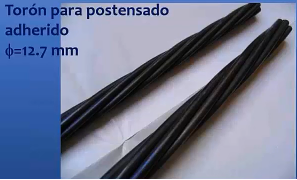
\includegraphics{4.png}
\end{figure}

Para el \textquotedbl sistema no adherido\textquotedbl se utiliza el mismo cable pero esta recubierto
con grasa y una capa de plastico.

\begin{figure}[H]
\centering
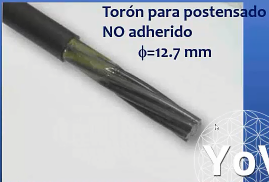
\includegraphics{5.png}
\end{figure}

El diametro que más se utiliza es el de media pulgada o de 12.7 mm, en los catalogos
de los fabricantes se puede encontrar direfentes diametros pero el de diametro 12.7mm
es el mas comercial.

\section{DETALLE CABLE PARA POSTENSADO NO ADHERIDO}

\begin{figure}[H]
\centering
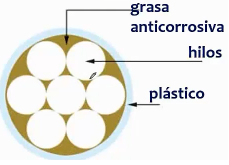
\includegraphics{6.png}
\end{figure}

Se puede apreciar que es un toron de siete hilos recubierto con una capa de plastico
y engrasado, nosotros le decimos engrasado y envainado.

\begin{figure}[H]
\centering
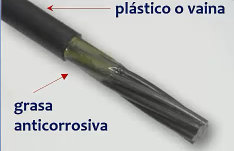
\includegraphics{7.png}
\end{figure}

Una vez que se realiza el tesado en una losa postensada no se requiere inyección
de lechada

\section{DETALLE CABLE PARA POSTENSADO NO ADHERIDO}

\begin{itemize}
	\item El cable viene en bobinas de 2 a 2.5 toneladas.
	\item El cable pesa 0.88 kg/ml
\end{itemize}

\begin{figure}[H]
	\begin{subfigure}{0.3\textwidth}
		\centering
		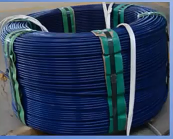
\includegraphics{8.png}
	\end{subfigure}
	\begin{subfigure}{0.3\textwidth}
		\centering
		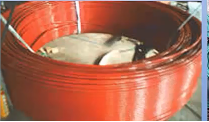
\includegraphics{9.png}
	\end{subfigure}
	\begin{subfigure}{0.3\textwidth}
		\centering
		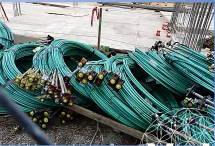
\includegraphics{10.png}
	\end{subfigure}
\end{figure}

Una de las ventajas de usar el diametro de media pulgada es que es flexible.
Podemos observar en la imagen que el material puede tener vainas de diferente
color, llegan en bobinas que pesan entre 2 a 2.5 toneladas.
El peso del cable incluyento la grasa es de 0.88 kg/ml.

\section{DETALLE ANCLAJES PARA POSTENSADO NO ADHERIDO}

\begin{itemize}
	\item {Anclaje mide 6.5 cm x 12.5 cm aprox. Puede ser activo (vivo)
	o pasivo (muerto). Consigue el efecto del postensado transmitiendo la 
	fuerza del cable a la masa de hormigón.}
	\item {Cuña de 2 piezas. Sujeta el cable al anclaje.}
	\item {Se colocan dos anclajes por toron.}
\end{itemize}

\begin{figure}[H]
\centering
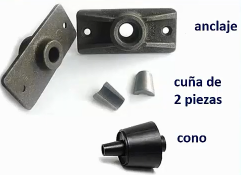
\includegraphics{11.png}
\end{figure}

El sistema que mas se utiliza es monotoron, se llama monotoron, porque
cada toron tiene su par de anclajes. Necesita un anclaje en cada extremo.
El cono lo ponemos al anclaje activo (lo llamamos vivo), para poder hacer
la limpieza despues del hormigonado, cuando se haya que tesar la losa.

Los que fabrican mejor los torones segun el Ing. Abner son los Estadounidenses.
y tambien son los mas economicos aunque paresca dificil de creer. Generalmente
el material hecho en china es mas economico, pero en este caso el material
Americano es más economico y es mejor.

\section{ANCLAJES ENCAPSULADOS PARA POSTENSADO NO ADHERIDO}

\begin{figure}[H]
	\begin{subfigure}{0.5\textwidth}
	\centering
	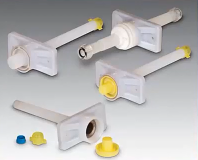
\includegraphics{12.png}
	\end{subfigure}
	\begin{subfigure}{0.5\textwidth}
	\centering
	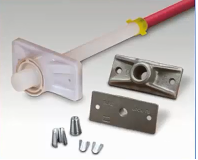
\includegraphics{13.png}
	\end{subfigure}
\end{figure}

Un problema en las estructuras que se hacen en la costa, a orillas del mar,
es el ataque o la corrosión que pueden sufrir los anclajes, en el acero en
general, se ha previsto eso, ahora se fabrican anclajes plastificados, estos
anclajes se recomienda en lugares agresivos. Respecto al costo los anclajes
cuestan de dos a tres veces el anclaje que no esta plastificado. Hablando de
las ciudades de Bolivia, no es necesario usar los anclajes plastificados.

\section{DETALLE DE ANCLAJE + CUÑA + CABLE}

\begin{figure}[H]
	\begin{subfigure}{0.5\textwidth}
	\centering
	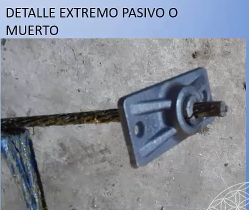
\includegraphics{14.png}
	\end{subfigure}
	\begin{subfigure}{0.5\textwidth}
	\centering
	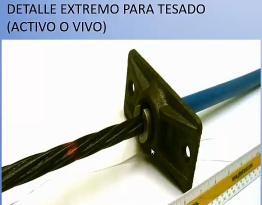
\includegraphics{15.png}
	\end{subfigure}
\end{figure}

Cada toron se instala dentro de la masa de hormigon, donde el extremo donde
tesamos el cable le llamamos \textquotedbl activo\textquotedbl o \textquotedbl vivo\textquotedbl
y el otro extremo le llamamos \textquotedbl pasivo\textquotedbl o \textquotedbl muerto\textquotedbl .
En el anclaje activo dejamos un pedazo libre de cable para que el gato hidraulico pueda sujeta y jalar
el cable, ese pedaso debe medir por lo menos 30 cm para que el gato hidraulico pueda realizar el tesado
sin ningun problema. En el extremo muerto no es necesario dejar el pedazo libre,
el extremo muerto se tesa en taller, antes de la instalación del toron dentro de la masa
de hormigon. El anclaje muerto se tesa con alrededor del 50\% de su capacidad.

\section{EQUIPO PARA POSTENSADO}

\begin{itemize}
	\item {El equipo es un circuito hidraúlico que proporciona una fuerza de
	       15 toneladas (cable de 12.7 mm) para estirar (tesar) el cable.}
	\item {El gato para postensado pesa 18 kg y la bomba puede pesar hasta
			20 kg.}
\end{itemize}

\begin{figure}
\centering
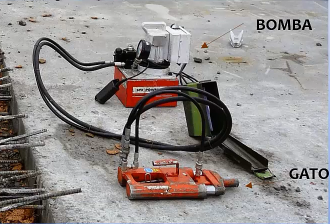
\includegraphics{16.png}
\end{figure}

Estos equipos han sido diseñados para trabajos en altura por lo livianos
que son, se puede trabajar en un piso 20, en un piso 30 debido a su bajo
peso, existen otros equipos mas pesados que son utilizados para losas
en pisos de poca altura, mientras mas liviano su uso puede ser para pisos
que estan a mayor altura, para trabajos en altura, el gato que vemos en
la figura puede tener una fuerza de tracción de 20 toneladas, pero
solo se requiere una fuerza de 15 toneladas para estirar los cables. El
losas postesadas.

\section{Precio solo del Gato de postensión}

\begin{figure}[H]
\centering
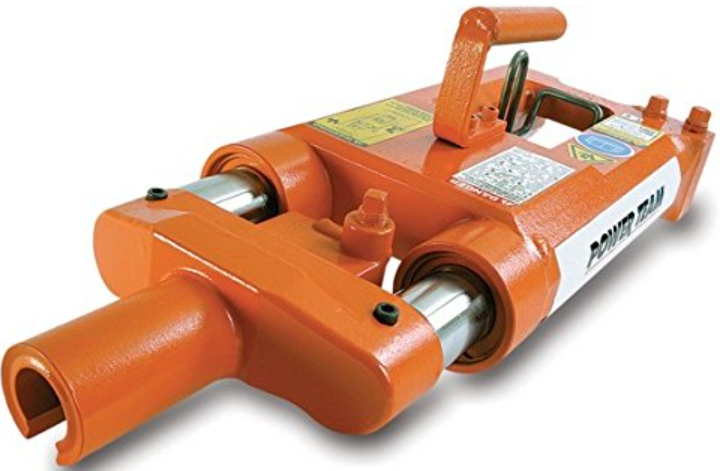
\includegraphics{17.png}
\end{figure}

SPX Power Team SJ2010DA Jack de tensión de poste de doble acción con
asiento eléctrico, 0.50 pulgadas, capacidad de 20 toneladas,
carrera de 8 1/2 pulgadas.

Marca: Marca: SPX POWER TEAM

\begin{verbatim}
Detalle de costo (Producto nuevo en amazon web):
Precio = 9213 usd
Importación = 2,239.96 usd
Total = 11453 usd (dolares americanos)
\end{verbatim}

\begin{verbatim}
Especificaciones para este Producto:
Capacidad de carga : 20 ton
Material : Acero
Peso del producto : 45 libras.
Preción operativa máxima : 10000 pounds_per_square_inch
Número de modelo : SJ2010DA
\end{verbatim}

\section{Precio solo de la bomba electrica}

\begin{figure}[H]
\centering
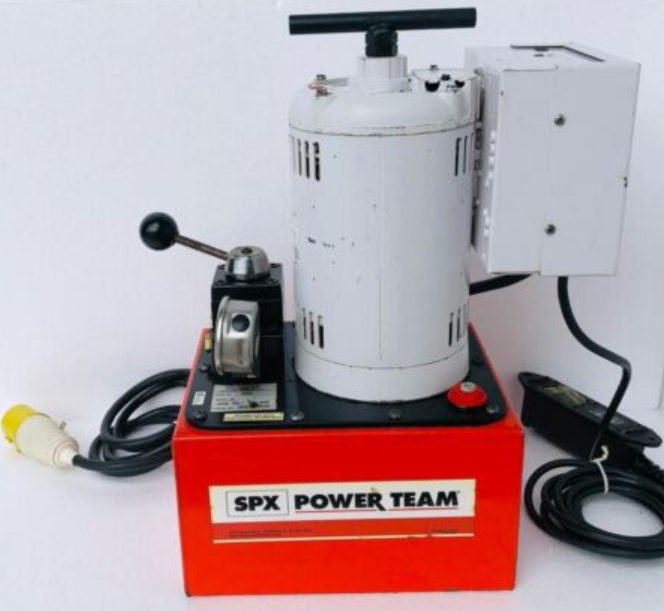
\includegraphics{18.png}
\end{figure}

Spx equipo de energía PE462 Bomba Hidráulica eléctrica/Power
Pack 4 vías Válvula 230V

\begin{verbatim}
Producto Nuevo.
Total = 8850 usd (dolares americanos)
\end{verbatim}

\begin{verbatim}
Especificaciones para este Producto:
Estado del artículo : Nuevo
Rated Pressure : 10000 psi (700 bar)
Power Source : Electric
Brand : SPX POWER TEAM
Pump Action : Double Acting
\end{verbatim}

\section{POSICION DEL CABLE EN LA LOSA DE HORMIGON}

\begin{figure}[H]
\centering
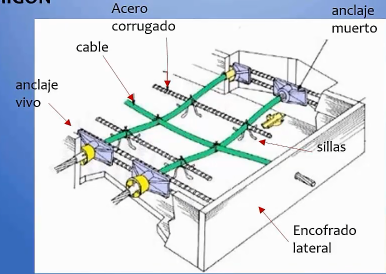
\includegraphics{19.png}
\end{figure}

Para darle la trayectoria o perfilado a los tendones vamos
a usar barras corrugadas, se puede apreciar en la imagen las
llamadas sillas que son de acero corrugado y tambien las barras
que van de silla a silla en la imagen y que son de 12 mm de
diametro en una losa llena para poder soportar el peso
del obrero.

La separación máxima de las sillas (un metro), tambien se
puede ver en la imagen los conos que estan dibujados de color
amarillo, una vez que el hormigon ha alcanzado la resistencia
adecuada estos conos se retiran y se realiza el tesado de los
cables.

\section{POSICION DEL CABLE EN LOSAS Y VIGAS DE FUNDACION}

\begin{figure}[H]
\centering
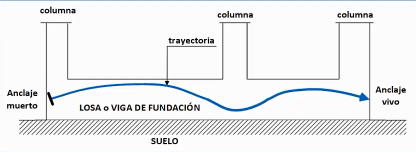
\includegraphics{20.png}
\end{figure}

La trayectoria en el caso de una fundación postensada es inversa.

\section{ELEMENTOS USADOS PARA DAR LA TRAYECTORIA AL CABLE}

\begin{itemize}
	\item Las sillas deben ser de diferentes alturas.
	\item {Las sillas pueden ser fabricadas en obra o prefabricadas
		(de plástico adecuado)}
	\item Es conveniente usar prefabricados para alturas pequeñas.
\end{itemize}

\begin{figure}[H]
	\begin{subfigure}{0.5\textwidth}
	\centering
	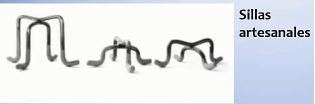
\includegraphics{21.png}
	\end{subfigure}
	\begin{subfigure}{0.5\textwidth}
	\centering
	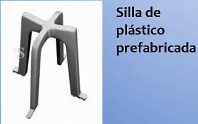
\includegraphics{22.png}
	\end{subfigure}
\end{figure}

\section{Losa llena (maciza)}

\begin{figure}[H]
\centering
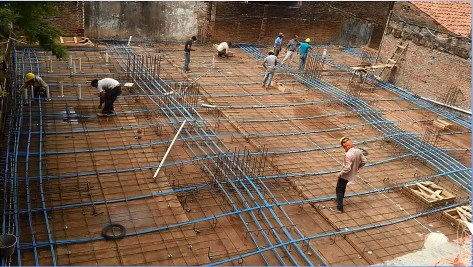
\includegraphics{23.png}
\end{figure}

En los sectores donde se ven tendones agrupados
se les llama bandas, se acemejan a vigas. y en la otra dirección
estan los tendones distribuidos, se acemejarían a viguetas.

Puede haver solo bandas en una losa, tambien puede darse el
caso de que solo haya tendones distribuidos en una losa.

Pero esta combinación de bandas y en el otro sentido tendones
distribuidos es el arreglo mas optimo al que se ha llegado.

\begin{figure}[H]
\centering
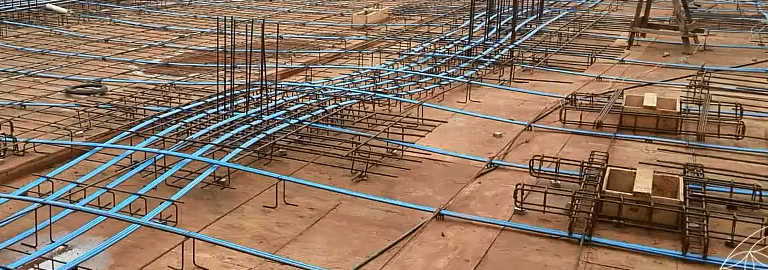
\includegraphics{24.png}
\end{figure}

Ahora vemos un detalle de losa llena en la zona de los anclajes
activos.

\begin{figure}
\centering
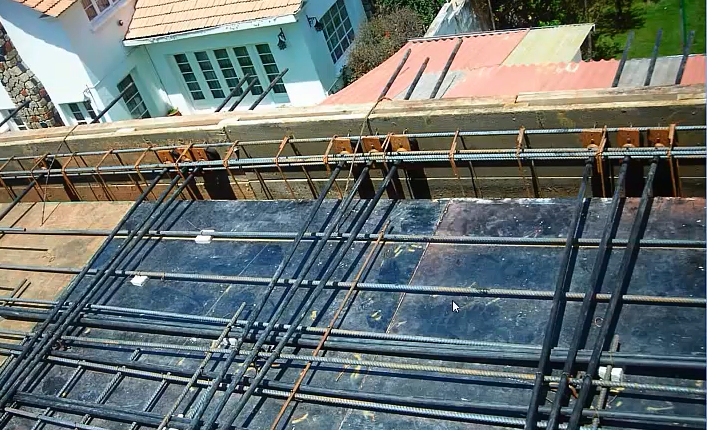
\includegraphics{25.png}
\end{figure}

El instituto del postensado recomienda en losas llenas que como
minimo se coloque 2 cables en la zona de tendones distribuidos.

Por otro lado se puede notar en la imagen que las instalaciones
electricas estan dentro de la masa de hormigon (dentro de la
losa maciza.)

\begin{figure}[H]
\centering
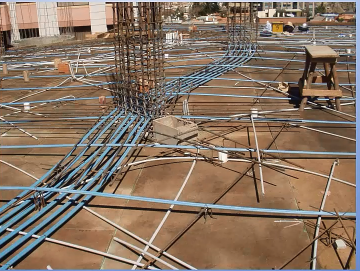
\includegraphics{26.png}
\end{figure}

Hay una malla inferior distribuida (barras corrugadas) que como
armadura minima exige la norma europea, pero la norma americana
no exige dicha malla inferior. Por otro lado en el borde de losa
donde se encuentran las los anclajes activos la norma europea
recomienda una vigas de borde, es decir cuatro barras y estribado
formando una viga de borde mientras que en la norma americana
solo se exige dos barras de 12 mm.

En las ciudades como La Paz y el Alto el hormigon alcanza la
resistencia de 21 Mpa a los siete dias mientras que en las ciudades
como Cochabamba y Santa Cruz se alcanza un hormigon con resistencia
especificada de 21 Mpa al tercer o cuarto dia. Una vez que se hace el
tesado ya se puede retirar el encofrado de losa, solo hay que dejar unos
cuantos puntales.

En losas postesadas aligeradas tambien se recomienda por parte del
instituto del postesado poner 2 cables, y vemos que estos nervios
tienen una separación de un metro.

La tolerancia en la elongación del cable es de mas menos siete por
cientos. Luego se corta el cable sobrante y se tapa con un plastico
el hueco de los anclajes para su sellado con mortero y aditivo
para que expanda el mortero y evitar ataque de agentes quimicos, luego queda asi
durante toda su vida util, no se necesita mantenimiento esta losa, no
se necesita hacer un retesado durante la vida útil de la losa.

La losa llena es la estrella de las losas postensadas por su velocidad de
ejecución y su versatilidas para lograr geometrias complejas en planta.

Las experiencias del Ing. Abner construyendo losa en la ciudad de La Paz
con columnas separadas 8 m de uso residencial logrando construirse con
una losa llena de 20 cm de espesor y con un hormigon con una resistencia
especificada de 28 Mpa.

\section{TIPOS DE LOSAS POSTENSADAS (LOSAS LLENAS CON CAPITELES)}

\begin{itemize}
	\item Luces hasta 13 m
	\item Se adapta a geometrias complejas
	\item {Cargas ligeras a pesadas (unidades habitacionales, parqueos
		de vehiculos grandes, jardines y otros.}
\end{itemize}

\begin{figure}[H]
	\begin{subfigure}{0.5\textwidth}
	\centering
	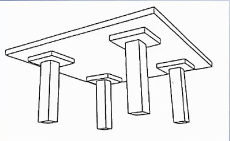
\includegraphics{27.png}
	\end{subfigure}
	\begin{subfigure}{0.5\textwidth}
	\centering
	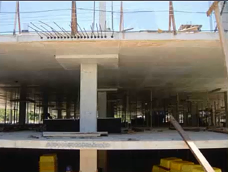
\includegraphics{28.png}
	\end{subfigure}
\end{figure}

Se aconseja que el espesor del capitel, es decir por debajo de la losa
llena no sea menor a 15cm por facilidad constructiva.

Es decir no es necesario aumentar el espesor de toda la losa
simplemente aumentar capiteles en la zona de las columnas.

\section{LOSAS ALIGERADAS EN DOS DIRECCIONES O TIPO WAFFLE}

\begin{itemize}
	\item Luces hasta 14 m
	\item {Cargas ligeras a pesadas (unidades habitacionales,
		parqueos de vehiculos grandes, jardines y otros.)}
\end{itemize}

\begin{figure}[H]
	\begin{subfigure}{0.5\textwidth}
	\centering
	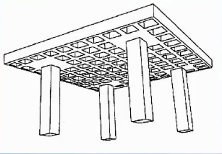
\includegraphics{29.png}
	\end{subfigure}
	\begin{subfigure}{0.5\textwidth}
	\centering
	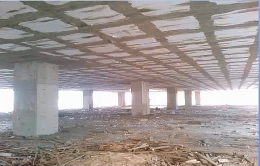
\includegraphics{30.png}
	\end{subfigure}
\end{figure}

Nos damos cuenta que hemos llegado al limite de la luz entre
columnas, es decir a la longitud de la losa con lo que en las
armaduras empiezan a incrementar considerablemente, o la carga
es muy grande para la losa, entonces hay que buscar otra
alternativa, entonces nos damos cuenta que la losa requiere
mucho acero adherido o mucho cable, entonces se busca otra
alternativa de solución.

Las losas aligeradas en comparación a las losas llenas
son mas lentas de ejecutar, es decir que las losas llenas
son mas rapidas de construir, otra obserbación es que entra
mas acero adherido en una losa aligerada que en una losa llena,
pero en una losa aligerada entra menos cable.

video en espera min 53:00
